% Second revision (round 2) response letter, Manuscript LR20628MR.
% DRAFT. Red \todo{} markers flag items that still need a decision, an
% analysis, or a manuscript change. Remove the \todo macro's output
% (set \todoon to false below) before submission.
\documentclass[11pt]{article}
\usepackage[margin=1in]{geometry}
\usepackage[colorlinks=true,allcolors=blue]{hyperref}
\usepackage{xcolor}
\usepackage{amsmath}
\usepackage{graphicx}
\renewcommand{\figurename}{Response Figure}

% Manuscript notation, so text drawn from bv-methods-review reads the same here.
\newcommand{\sij}{S_{ij}}
\newcommand{\Ro}{R_0}
\newcommand{\Rij}{R_{ij}}

\newenvironment{refquote}%
  {\begin{quote}\itshape\color{black!70}}%
  {\end{quote}}

% Draft markers. Set \todoon to false to suppress them in the final letter.
\newif\iftodoon
\todoontrue
\newcommand{\todo}[1]{\iftodoon{\color{red}\bfseries[TODO: #1]}\fi}

\setlength{\parskip}{0.5\baselineskip}
\setlength{\parindent}{0pt}

\begin{document}

\begin{center}
{\large\bfseries Response to the Referees --- Second Revision}\\[2pt]
Manuscript LR20628MR --- ``Yukawa screening derivation of the bond-valence rule''
\end{center}

We thank both referees.  The First Referee, whose first-round report
shaped the previous revision, now recommends publication.  The Second
Referee is new to the manuscript and raises concerns in four areas.
These are the alternative empirical forms of the bond-strength law and
the notation of the expansion point, the construction and
interpretation of manuscript Fig.~1 and the Supplemental figures of $B$--$R_0$
lines, the physical motivation for expanding about the Gibbs mean in
the partition-thermodynamics section, and the transferability of the
bond-valence parameters when each structure is fitted individually.
We respond to each point below.

\textbf{Summary of changes.}  Five passages of the manuscript were
changed in response to the Second Referee, all in the main text and
all marked in the accompanying tracked changes.  First, the sentence
after Eq.~(3) was reworded to remove the ambiguity the referee read as a
typographical error (Block~3a).  Second, a clause after Eq.~(4) now
identifies $B$ as the inverse log-weight slope at the expansion
point, and the sentence introducing Eq.~(5) states that the
uniform-limit relation follows from Eq.~(1) alone (Block~3b).  Third,
a statement after Eq.~(5) makes explicit that the predicted slope
describes the family of per-structure fits rather than prescribing a
single pair (Block~6).  Fourth, the Partition thermodynamics section
closes with the physical argument for expanding about the Gibbs mean
(Block~8).  Fifth, the paragraph after Eq.~(4) now places the
Brown--Shannon power law as the same screened weight linearized in
$\ln R$, with four references added (Block~2).  Two figures were
prepared for this response.  Response
Figure~\ref{fig:lambda_hist} shows the distribution of the
per-structure screening length across the corpus, and Response
Figure~\ref{fig:co_points} redraws the Co--O panels of Supplemental
Fig.~S4 with the underlying per-structure points.  Every statistic
quoted in this letter is reproduced by scripts in the project
repository \cite{YukawaScreeningRepo}.  In the Supplemental Material, the fifteen coordination-resolved
$B$--$R_0$ line figures (Figs.~S2--S16) were regenerated to show the
per-structure points within a physical window, with the convention
stated in the text, and the Data provenance section now states the
stability filter.

\section*{Second Report of the First Referee}

\begin{refquote}
``The authors have substantially improved their manuscript and I can
now recommend publication.''
\end{refquote}

\textbf{Response.}  We thank the referee for the careful first-round
report and for this recommendation.

\section*{Report of the Second Referee, with responses}

\begin{figure}[!b]
\centering
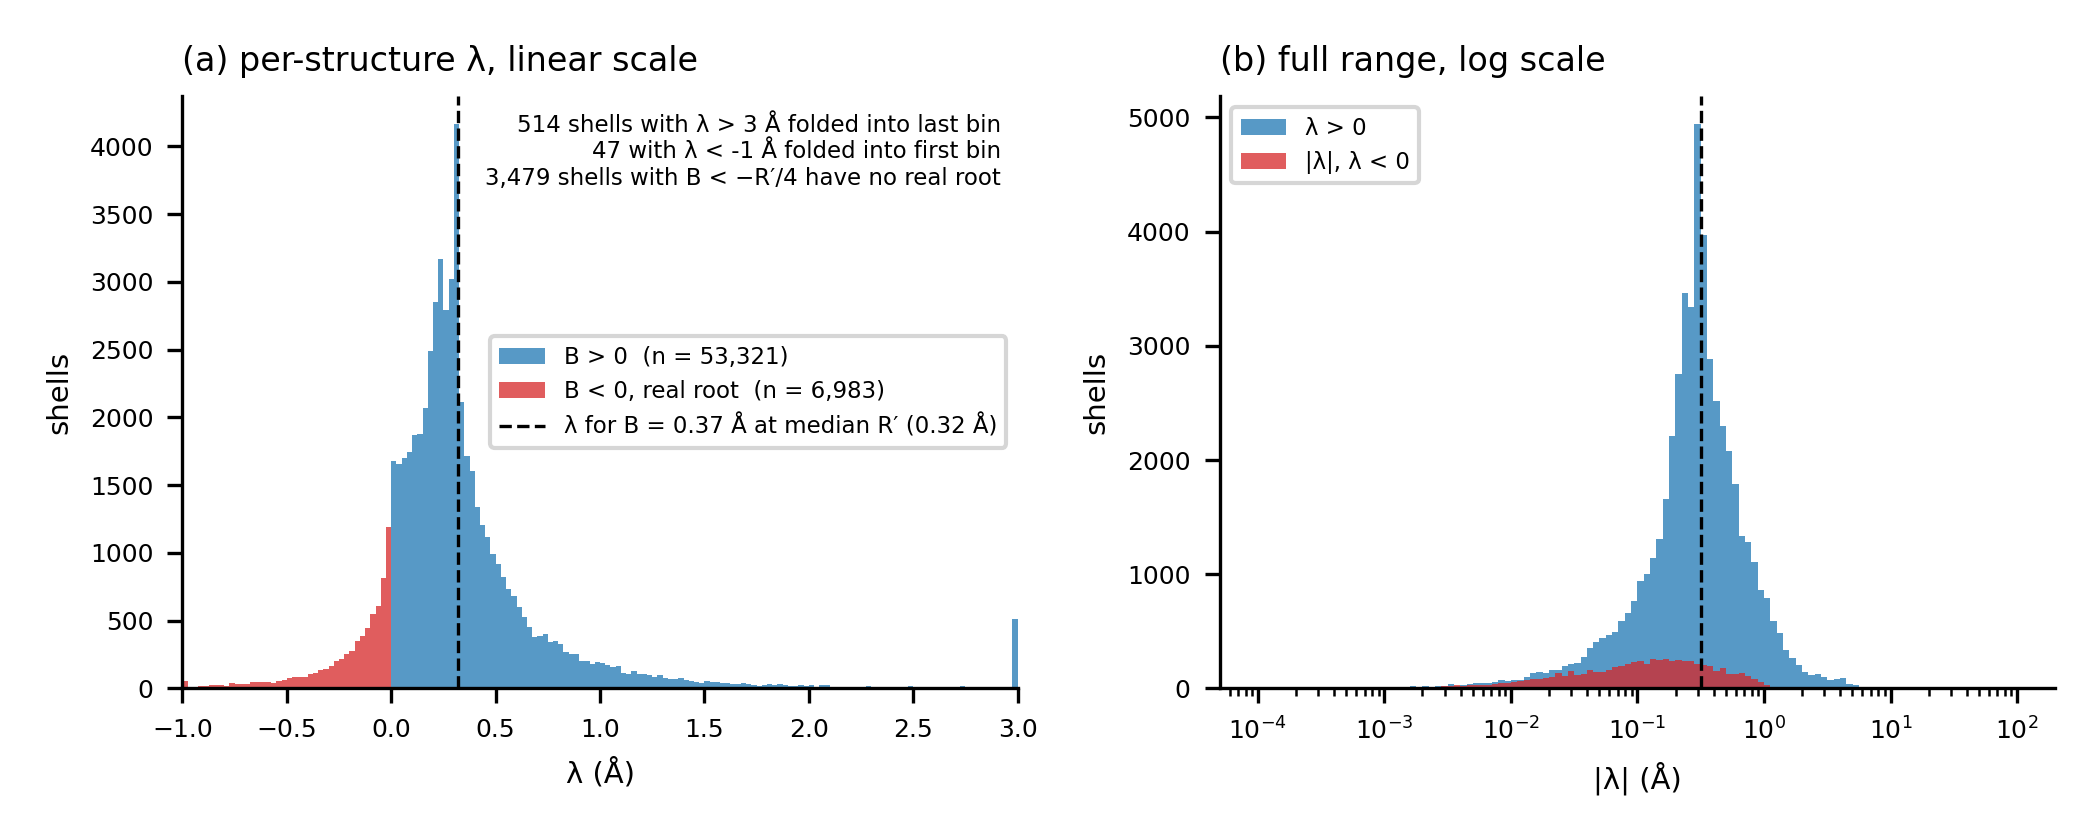
\includegraphics[width=\textwidth]{response_figures/lambda_per_structure_hist.png}
\caption{Per-structure Yukawa screening length
$\lambda=(-R'+\sqrt{R'^2+4BR'})/2$, with $R'$ the shell's mean bond
length, for all 63{,}783 single-valence fitted cation--oxygen shells
in the corpus.  (a) Linear scale from $-1$ to $3$~\AA.  Blue, the
screening branch $B>0$ (53{,}321 shells).  Red, the anti-screening
branch $B<0$ where the root is real (6{,}983 shells).  The 514 shells
with $\lambda>3$~\AA{} and 47 with $\lambda<-1$~\AA{} are folded into
the end bins, and the 3{,}479 shells with $B<-R'/4$ have no real root.
The dashed line is $\lambda$ for the conventional $B=0.37$~\AA{} at
the corpus median bond length of $2.02$~\AA.  (b) The same values as
$|\lambda|$ on a logarithmic axis over the full range.}
\label{fig:lambda_hist}
\end{figure}

\textbf{Block 1 --- introductory remarks.}

\begin{refquote}
``The manuscript proposes a theoretical basis for calculating bond
strength in bond-valence theory, deriving the bond strength from the
electrostatic flux associated with a Yukawa potential.  Bond-valence
theory is an empirical framework widely used in materials science,
particularly for the validation of crystal structures and the study
of ion diffusion in solid-state ionic conductors.  I believe that this
could be an interesting topic for the readers of Physical Review
Materials.

However, I did not find the manuscript particularly convincing.  The
exposition is not always clear, some aspects of the theoretical
framework are not sufficiently justified, and I have serious concerns
about the validity of some of the calculations presented, as well as
about the interpretation of some of the figures.''
\end{refquote}

\textbf{Response.}  We thank the referee for the assessment of the
topic and for a report whose specific concerns we can act on.  

The referee's central worry, developed in Blocks~5 through~7 and in the
closing remarks, is that the per-structure $(R_0,B)$ values span
ranges that appear unconventional.  We clarify the relationship
between the bond-valence convention and its physical underpinning.
Although $(R_0,B)$ are conventionally read as a reference bond length
and a softness length, no prior theory bounds the values they may
take.

Our position is that bond valence theory is an approximation, and the
application of it to a large corpus of structures will identify materials that do 
not conform to the assumptions of the approximation. The conventional approach has 
often relied on carefully curated data sets from which non-conforming structures were removed. 
For example, one seminal study eliminated about 15\% of the alkali coordinations in its
reference set, relative to the 1{,}524 retained for the final refinements,
because of their ``strange bond-valence sums'' \cite{Adams2001}.
This carries a risk of circularity, since selecting structures that
conform to the theory is not a test of its applicability, and some of
the structures whose per-structure fits look ``strange'' are very
common ground-state ones, such as the nearly degenerate SiO$_2$ polymorphs
discussed in the manuscript's screening-collapse section.  Here, we instead
force the theory to confront a large set of DFT-relaxed structures from the
Materials Project, a database in wide community use, screened for
thermodynamic stability as described under Block~7. 
Letting the poor fits mark the limits of the approximation is part
of the result, and it points towards a physical basis for the
parameters.  Specifically, we test bond valence theory against DFT and show exactly where it fails,
pointing to specific failure mechanisms (lone pairs, Jahn--Teller physics) 
rather than omitting failures from the fit and leaving their status ambiguous.

The new physical content we present is the screening length, and it
does not suffer from the extreme values that the per-structure
$(R_0,B)$ can take.  Response Figure~\ref{fig:lambda_hist} shows the
per-structure $\lambda=(-R'+\sqrt{R'^2+4BR'})/2$, with $R'$ approximated here 
as the mean bond length of the shell, for all 63{,}783 single-valence fitted
shells in the corpus.  On the screening branch ($B>0$, 84\% of
shells) $\lambda$ is a single peak with median $0.30$~\AA{} and
interquartile range $0.18$--$0.47$~\AA, 95\% of the values lie below
$1.2$~\AA, and only 1\% exceed $3$~\AA.  Along the degenerate
direction of the $(R_0,B)$ plane the inversion of Eq.~(4) gives
$\lambda\simeq\sqrt{BR'}$, so a $B$ of $10^{3}$~\AA{} becomes a
$\lambda$ of about $45$~\AA{} and the tail is compressed by two
orders of magnitude.  The conventional $B=0.37$~\AA{} corresponds to
$\lambda=0.32$~\AA{} at the median bond length, at the center of the
peak.  The anti-screening branch ($B<0$) is 16\% of shells.  Of these,
11\% of all shells have a real root, with median $\lambda=-0.12$~\AA,
and 5\% have $B<-R'/4$ and no real root, which marks where the
first-order Yukawa form ceases to apply.  The species-level
$\lambda^*$ tabulated in the Supplemental Material (median
$0.31$~\AA, interquartile range $0.26$--$0.37$~\AA) sit at the center
of this per-structure distribution.



\textbf{Block 2 --- alternative empirical forms of the bond-strength
law.}

\begin{refquote}
``The derivation of the bond strength from a Yukawa potential is
interesting.  It is an extension of a previous idea that linked
electrostatic flux with bond strength.  This work shows that when the
electrostatic flux is derived from a Yukawa potential, the empirical
exponential form of the bond strength is recovered.  However, there
are other empirical forms that also work well, such as the original
power-law relationship introduced in the original formulation of
bond-valence theory by Brown and Shannon (Acta Cryst.\ A29, 266--282,
1973).  The manuscript neither mentions nor discusses these
alternative formulations, which give different dependencies of the
bond strength on the bond distance.''
\end{refquote}

\textbf{Response.}  The referee is right that the power-law form has
been used previously in the literature. 
Brown and Shannon \cite{Brown1973} fitted individual
curves $S=s_0(R/R_0)^{-N}$ and universal curves $S=(R/R_1)^{-N}$,
with $R_1$ the length of a bond of unit valence and $N$ between
$4.1$ and $6.1$ for the isoelectronic cation series, building on the
per-polyhedron power-law curves of Donnay and Allmann
\cite{Donnay1970}.  Brown and Wu \cite{Brown1976} tabulated
$(R_1,N)$ for cation--oxygen pairs, and the power law was in routine
use through the 1970s.  Zachariasen \cite{Zachariasen1978} compared
it with the logarithmic form $D(s)=D(1)-B\ln s$, which is Eq.~(1)
solved for the bond length, and found that the two agree to better
than $1\%$ for $0.5<s<2$ when $N=D(1)/B$, but differ by $5$--$7\%$
in bond length at $s=0.1$.

In fact, the two forms are not in competition within the limits of the approximation.  
Both are leading-order expansions of the same
Yukawa log-weight, taken in different variables.  Expanding
$\ln w_{ij}$ in $R_{ij}$ about $R'$ gives the exponential of
Eq.~(1) with $B=\lambda(\lambda+R')/R'$, which is Eq.~(4).
Expanding the same $\ln w_{ij}$ in $\ln R_{ij}$ about $\ln R'$ gives
the power law, because
\[
\frac{d\ln w}{d\ln R}
=-\frac{(R/\lambda)^2}{1+R/\lambda},
\qquad\text{so}\qquad
N=\frac{R'^2}{\lambda(\lambda+R')}=\frac{R'}{B}.
\]
This is Zachariasen's condition $N=R_1/B$ for the two forms to
coincide \cite{Zachariasen1978}, obtained here as the ratio of the
two leading-order expansions of one screened weight.  With
$B\simeq0.37$~\AA{} and the Brown--Shannon $R_1\simeq1.4$--$1.8$~\AA{}
it gives $N\simeq4$--$5$, in the range of their universal exponents.
The exponential is
the form that is linear in the bond length, which is why it is the
one whose $B$--$R_0$ correlation has a parameter-free slope, but the
power law is the same screened weight linearized in the logarithm of
the bond length.

We retain the exponential form because it is linear in the bond
length, which is what gives the $B$--$R_0$ correlation its
parameter-free slope.

\emph{Changes.}  The manuscript now discusses the power law.  After
Eq.~(4) it states: ``The power-law form $S=(R/R_1)^{-N}$ of Brown and
Shannon \cite{Brown1973}, which traces to Donnay and Allmann
\cite{Donnay1970} and was tabulated for cation--oxygen pairs by Brown
and Wu \cite{Brown1976}, is the same screened weight linearized in
$\ln R$ instead of $R$, with exponent $N=R'/B$.  This is the condition
under which Zachariasen found the two forms to agree to within 1\%
for $0.5<S<2$ \cite{Zachariasen1978}.  We retain the exponential
because it is linear in the bond length, which is what gives the
$B$--$R_0$ correlation below a parameter-free slope.''  The four
references were added to the manuscript bibliography.

\textbf{Block 3 --- minor remark on $R'$ versus $R_0$.}  The
referee's remark contains two questions, answered separately.

\textbf{Block 3(a) --- is ``at $R_{ij}=R'$'' a typographical error?}

\begin{refquote}
``A minor remark.  After linearizing the weights (Eq.~3), the authors
state: `Exponentiating the linear term and renormalizing therefore
reproduces Eq.~1 at $R_{ij}=R'$.'  I suspect this is a typographical
error, and that the authors actually mean $R'=R_0$ because this is
the choice that reproduces Eq.~1.''
\end{refquote}

\textbf{Response.}  It is not a typographical error, but the sentence
was ambiguous and we have reworded it to improve clarity.  Exponentiating the linear
term of Eq.~(3) and renormalizing reproduces the exponential form of
Eq.~(1) for every bond in the shell, whatever the expansion point.
What the expansion point sets is where the linearized weight equals
the exact Yukawa weight.  The phrase ``at $R_{ij}=R'$'' meant that
the error $\delta_{ij}$ vanishes at that bond length and grows
quadratically away from it.  It was not a statement about $R_0$.
The choice $R'=R_0$ would not make Eq.~(1) exact anywhere in
particular, because $R_0$ is in general not a bond length of the
shell.  It is the intercept of Eq.~(1), and the partition identity of
Eq.~(10) shows that it differs from the valence-weighted shell
centroid $m_i$ by the entropy correction $B(\ln q_i-H_i)$, which in
the uniform-bond limit is $B\ln(z/n)$.  The two lengths coincide
only for a single bond of unit valence, the Brown limit noted after
Eq.~(10).

\emph{Changes.}  The sentence after Eq.~(3) now reads
``Exponentiating the linear term and renormalizing reproduces the
exponential form of Eq.~(1).  The log-weight error vanishes at
$R_{ij}=R'$ and is quadratic away from it.''

\textbf{Block 3(b) --- why $R'$ appears in Eq.~4, and whether Eq.~5
assumes $R'=R_0$.}

\begin{refquote}
``Why is $R'$ used in Eq.~4 rather than $R_0$?  In Eq.~5, the authors
calculate $dB/dR_0$ from Eq.~4, which appears to implicitly assume
that the $R'$ in Eq.~4 is in fact $R_0$.''
\end{refquote}

\textbf{Response.}  $R'$ appears in Eq.~(4) because $B$ is defined
there as the inverse of the local slope of the Yukawa log-weight,
$-d\ln w/dR=R/[\lambda(\lambda+R)]$, evaluated at the expansion
point.  That slope depends on where in the shell the expansion is
centered, so the composite $B=\lambda(\lambda+R')/R'$ necessarily
carries $R'$.  Replacing $R'$ by $R_0$ would evaluate the slope at a
length that is not in the shell.

Equation~(5) is not derived from Eq.~(4) and makes no use of $R'$,
so no identification $R'=R_0$ is assumed.  It follows from applying
the valence-sum rule to Eq.~(1) in the uniform-bond limit, which
gives $R_0=\bar R+B\ln(z/n)$, and differentiating at fixed
$\bar R$.  The uniform-bond limit also shows directly that $R'$ and
$R_0$ differ.  With all $R_{ij}=\bar R$ the expansion point is the
shell radius, $R'=\bar R$, while $R_0=\bar R+B\ln(z/n)$ equals it
only at $z=n$.  Equation~(4) enters only when the fitted $B$ is read
as a screening length, and there the manuscript states the
operational choice of $R'$ explicitly.  Within a shell the
partition-thermodynamics section fixes $R'=m_i$, the Gibbs mean.

\emph{Changes.}  The sentence introducing Eq.~(5) now states that
the uniform-limit relation follows from the valence-sum rule applied
to Eq.~(1), involves only the fitted parameters, and uses nothing
from Eq.~(4).  A clause after Eq.~(4) now identifies $B$ as the
inverse of the log-weight slope $-d\ln w/dR=R/[\lambda(\lambda+R)]$
evaluated at the expansion point $R'$.

\textbf{Block 4 --- construction of manuscript Figure~1.}

\begin{refquote}
``I do not clearly see how Figure~1 has been calculated.  My
understanding is the following.  For a given A--O pair, the authors
have analyzed several crystal structures containing A--O
interactions, obtaining one pair $(R_0,B)$ for each structure.  When
$B$ is plotted against $R_0$, a strong linear correlation is found for
structures with the same coordination number.  The slope of this
linear correlation is $1/\ln(z/n)$.  Figure~1 appears to have been
constructed from the data shown in Figure~S2.  If I have understood
this correctly, I have several concerns.''
\end{refquote}

\textbf{Response.}  The referee's understanding is correct, with two
small refinements.  Each DFT-relaxed structure contributes one
jointly fitted $(R_0,B)$ pair.  For each species and coordination
number $n$ the pairs are regressed by an outlier-robust RANSAC
estimator refit on its inliers, and the slope of that regression is
one point of manuscript Fig.~1.  The lines drawn in the Supplemental figures are
these regressions, so manuscript Fig.~1 is built from the lines of
Figs.~S2--S16, not of Fig.~S2 alone.  The construction is described
in the manuscript (Empirical validation) and in the Supplemental
Material (``Line-fitting procedure'').  The prediction of Eq.~(5) is
that the slope of the per-structure correlation is $1/\ln(z/n)$ with
no fitted constants.

\textbf{Block 5 --- (a) range of the $R_0$ and $B$ values in the
Supplemental line figures.}

\begin{refquote}
``The ranges of $R_0$ and $B$ shown in Figure~1 are extraordinarily
large.  One would normally expect $R_0$ to be of the same order of
magnitude as the characteristic bond distance.  Taking Co--O as an
example, for Co$^{+1}$--O, $R_0$ appears to vary between
approximately 0 and 200~\AA; for Co$^{2+}$--O, between approximately
$-10$ and 10~\AA; and for Co$^{3+}$--O, between approximately $-1000$
and 1000~\AA.  These values do not appear physically meaningful.  The
parameter $B$ presents a similar problem.  In conventional
bond-valence parameterizations, $B$ is typically of the order of
$10^{-1}$~\AA.  In the case of Co$^{3+}$--O, for example, the values
shown in the figure appear to range from approximately -1000 to
1000~\AA.  Moreover, several of the curves extend into the region of
negative $B$ (anti-screening according to the formulation presented
in the manuscript, so bonding forces are increasing with bond
distance).

A further issue is that the individual $(R_0,B)$ values obtained from
the different crystal structures do not appear to be shown in
Figure~1.  Instead, only the least-squares regression lines are
displayed.  Why are the individual fitted $(R_0,B)$ pairs not shown?
I think it is important to show them explicitly, this would allow the
reader to assess the actual distribution of the fitted parameters,
the quality of the linear correlations, and the extent to which the
regression lines are representative of the underlying data.  I wonder
whether these extraordinarily large ranges could result from an error
in the way the curves are represented or plotted.  If this is indeed
the case, it would be rather surprising that such an issue was not
identified during the preparation or checking of the figures, even
though they are included in the Supplementary Material.  The authors
should therefore carefully verify the numerical values and the
plotting procedure used to generate these curves.''
\end{refquote}


\textbf{Response.}  We agree that there are extreme values that look
surprising, and we regret that the original figures did not portray
these values clearly, as they are portrayed in the
preceding manuscript on the method \cite{Li2025}.
Response Figure~\ref{fig:co_points} reproduces the four Co--O panels of
Supplemental Fig.~S4 with the per-structure $(R_0,B)$ pairs drawn
under the fitted lines, both at the full range of the fitted values
and within a restricted window, and all Supplemental line figures
(Figs.~S2--S16) have been regenerated with the per-structure points
in the same window.

We note that the large majority of structures have $(R_0,B)$ in
conventional ranges.  Of the 63{,}783 single-valence shells in the
corpus, 92\% lie within $0<R_0<4$~\AA{} and $-1<B<2$~\AA, and 74\%
within $0<R_0<4$~\AA{} and $0<B<1$~\AA.  For the Co species of
Response Figure~\ref{fig:co_points} the in-window fractions are 80\%, 89\%,
67\% and 93\% for Co$^{1+}$ through Co$^{4+}$.  The 8\% of shells
outside the window is below the roughly 15\% of coordinations that
were eliminated from another reference set for ``strange bond-valence
sums'' \cite{Adams2001}.  

Values in the tails are not outliers in the sense of being poorly
fitted or subject to numerical error.  They are degenerate.  For a
nearly regular shell, Eq.~(1) and the valence-sum rule constrain the
joint fit of $(R_0,B)$ only along the line $R_0=\bar R+B\ln(z/n)$,
and with equal bond lengths $B$ is unconstrained altogether.  The
second-order terms $\delta_{ij}$ of Eq.~(3) select a point on that
line, but when the bond-length spread is a few hundredths of an
\aa ngstr\"om the selection is weak and the least-squares solution
can lie along a wide range of the line, including at $|R_0|$ and $|B|$ of
order $10^{3}$~\AA.  

The data bear this out.  The shells outside the
window have a median bond-length range of $0.034$~\AA, against
$0.107$~\AA{} for those inside, and for Co$^{3+}$ at $n=6$ the
contrast is $0.023$ versus $0.283$~\AA.  Such a structure is an
inlier precisely because it lies on the line, and a structure fitted
at $(R_0,B)=(1000,700)$~\AA{} carries the same information about the
slope as one fitted at $(1.9,0.4)$~\AA{} and almost none about a
preferred point.  The referee is right that the individual values
are not meaningful as lengths.  The negative-$B$ segments arise in
the same way, since a line drawn across the full inlier range crosses
$B=0$ wherever the inliers straddle the shell radius, which is where
the line meets the axis by Eq.~(6).  The per-structure fits that
return $B<0$ are 16\% of the corpus, dominated by near-degenerate
shells, and are catalogued in the Supplemental sign census.  

This fit degeneracy is equally present in conventional fitting, which
suppresses it by fixing $B$ to a constant \cite{Brown1985} or by
pooling many structures to select one point in the shallow valley of
the residual surface \cite{Gagn2015}.  We include every structure
instead, not to assert that a $B$ of $10^{3}$~\AA{} is a physically
meaningful softness, but because such structures constrain the slope
that Eq.~(5) predicts as well as any other, and in order to be
transparent about the implications of applying the exponential
approximation universally.

\begin{figure}[htbp]
\centering
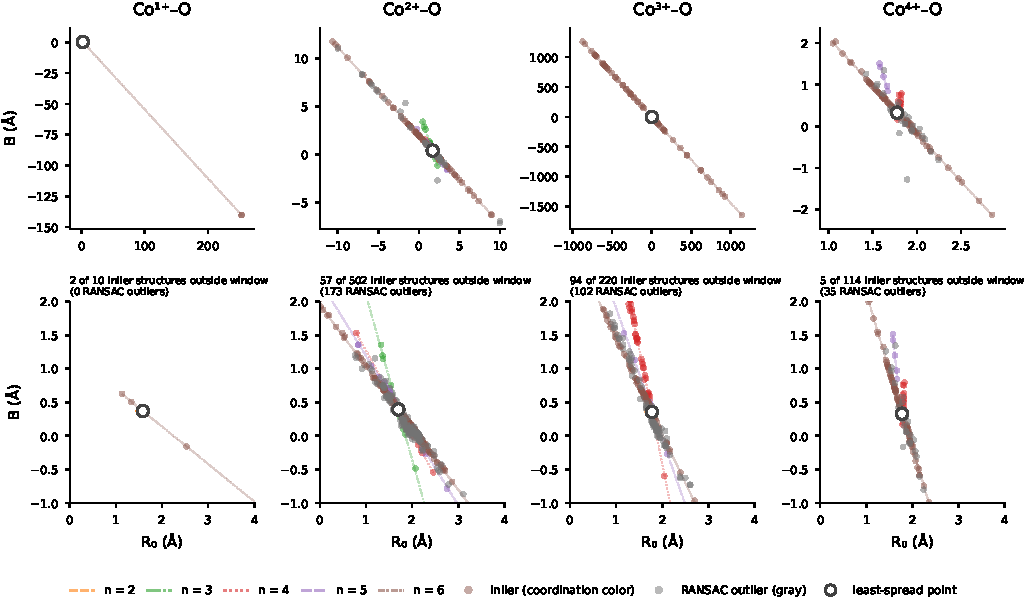
\includegraphics[width=\textwidth]{response_figures/co_o_fit_lines_with_points.pdf}
\caption{The four Co--O panels of Supplemental Fig.~S4 redrawn with
the per-structure $(R_0,B)$ pairs under the coordination-resolved
lines.  Top row, the full range of the fitted values, as plotted in
the Supplemental Material.  Bottom row, the same lines and points
within $0<R_0<4$~\AA{} and $-1<B<2$~\AA, with the number of inlier
structures outside the window stated above each panel.  Every per-structure
pair is a transparent filled circle, colored by coordination number
for RANSAC inliers and gray for RANSAC outliers.  Line styles encode
the coordination number $n$, and the open circle is the least-spread
intersection $(R_0^*,B^*)$.  Inlier and outlier counts are 10 and 0,
502 and 173, 220 and 102, and 114 and 35 for Co$^{1+}$ through
Co$^{4+}$.  The far-out points on the $n=6$ lines are shells with
nearly equal bond lengths, for which the joint fit is degenerate
along the line.}
\label{fig:co_points}
\end{figure}

\emph{Changes.}  Response Figure~\ref{fig:co_points} was prepared for
this response by re-running the Supplemental line-fitting pipeline
for the four Co species with the per-structure $(R_0,B)$ pairs
retained, so its lines are identical to those of Supplemental
Fig.~S4 (same seeded RANSAC fits, slopes and intercepts equal in all
13 species and coordination fits).  All Supplemental line figures (Figs.~S2--S16) have
been regenerated to show the per-structure $(R_0,B)$ pairs beneath
the fitted lines, with RANSAC inliers as filled circles and outliers
as open circles, axes fixed to $0<R_0<4$~\AA{} and $-1<B<2$~\AA,
and the number of inlier structures outside the window stated above
each panel.  The fitted lines are unchanged (slopes and intercepts
identical to the previous version for all 103 species).  The
Supplemental text introducing these figures now states the plotting
convention and explains the out-of-window structures.  The
corpus-wide and Co-specific statistics quoted above are reproduced by
two scripts added to the project repository
\cite{YukawaScreeningRepo}.  

\textbf{Block 6 --- (b) interpretation of the slope $dB/dR_0$.}

\begin{refquote}
``From the uniform bond limit, $R=R_0-B\ln(z/n)$, the authors derive
the slope $dB/dR_0=1/\ln(z/n)$.  They then use this equation to fit
the data in Figure~1.  If $R_0$ and $B$ in the uniform bond limit
equation are treated as variables, the above equation simply states
that there are infinite pairs $(R_0,B)$ that satisfy the valence-sum
rule for a regular coordination polyhedron with a given bond distance
and coordination number.

In my understanding, the uniform-bond limit is instead used to
determine the constant parameters $R_0$ and $B$ when a set of crystal
structures with regular coordination polyhedra is available, i.e.,
the variables are $R$ and $(z/n)$ and the constant parameters
obtained from the fit are $R_0$ and $B$.  The uniform bond limit
assumes that a series of structures can be described by a single
$(R_0,B)$ pair.  This is not the case in the authors' analysis, since
$R_0$ and $B$ are themselves treated as the variables defining the
correlation.

I do not question the observed linear correlation between $B$ and
$R_0$.  However, I do not believe that this linear relationship is
correctly derived from the uniform-bond limit.''
\end{refquote}

\textbf{Response.}  The referee's last sentence is the crux, so we
take it first.  The relationship is derived exactly.  For a shell
with every bond at $\bar R$, Eq.~(1) and the sum rule give
$n\exp[(R_0-\bar R)/B]=z$, that is $R_0=\bar R+B\ln(z/n)$, for every
$(R_0,B)$ that reproduces the structure.  The admissible pairs for
one regular structure therefore form a line through $(\bar R,0)$ with
slope $1/\ln(z/n)$.  The referee's own observation, that infinitely
many pairs satisfy the sum rule, is this line, and Eq.~(5) is its
slope.  Nothing is assumed about a series of structures sharing one
pair.

The prediction is where the per-structure fits must fall.  Each
structure is fitted alone and, if nearly regular, is confined to its
own line.  The lines of different structures at fixed species and
$n$ are parallel and offset by the spread in $\bar R$, about
$0.1$~\AA, while the fitted points spread along them over
\aa ngstr\"oms or more (Response Figure~\ref{fig:co_points}), so a
regression across structures recovers the common slope.  Manuscript
Fig.~1 tests that slope for 150 species and coordination pairs.  The
second-order terms of Eq.~(3) set where a distorted structure falls
on its line and produce the scatter treated in the near-pole
analysis.

The referee's reading is the conventional one, with $\bar R$ and
$z/n$ as the variables and one pair fitted across structures.  The
two uses do not conflict.  They are the same equation read along
different directions.  Conventional fitting picks one underdetermined
point on the line, which is why $B$ has usually been fixed.  We treat
the direction of the line as the physical content, because Eq.~(5)
predicts it with no adjustable constant.

\emph{Changes.}  The Parameter-free slope section now states, after
Eq.~(5), ``Equation~(5) does not prescribe a single $(R_0,B)$ for a
species.  It fixes the direction along which the joint fit of one
structure is degenerate, so the per-structure pairs of a species at
fixed $n$ trace a line of predicted slope and the second-order terms
set where each structure falls on it.''

\textbf{Block 7 --- (c) the $B$--$R_0$ correlation, published
variations of $B$, and structural validity.}

\begin{refquote}
``A final remark concerns the correlation between $R_0$ and $B$.  In
the authors' previous publication (Ref.~19 in the manuscript), it is
shown that the ranges of variation of $R_0$ and $B$ are still quite
large.  For instance, for Fe--O, $R_0$ varies from 0 to 4~\AA, while
$B$ varies from approximately $-2$ to $+2$~\AA.  In these figures the
data is shown as well as the fit.  I find these variations very
surprising.  Deviations from the commonly used value of $B=0.37$~\AA{}
have been investigated, for example, for Pb--O bonds by Krivovichev
and Brown (Z.\ Kristallogr.\ 216 (2001), 245--247), who found that
the Pb--O bonds were adequately described using $B=0.49$~\AA.  This
variation is much smaller than those reported by the authors.

I therefore wonder whether the structures used in the fits have been
carefully checked for their physical and structural validity.  If the
valence-sum rule is imposed on structures that are themselves
physically unrealistic, I imagine that the resulting bond-valence
parameters could be expected to show large deviations from the usual
values.  This possibility may be particularly relevant when working
with databases containing structures obtained from simulations rather
than from experimentally well determined crystal structures.''
\end{refquote}

\textbf{Response.}  The variations the referee quotes and the
variations in the published literature are different quantities.
The published values, including the $B=0.49$~\AA{} of Krivovichev and
Brown for Pb--O, are pooled per-pair fits, in which one pair
$(R_0,B)$ is chosen for all structures containing the pair.  Such a
fit selects one point in a shallow valley of the residual surface
whose floor runs along the line of Eq.~(5), and the choice between
$0.37$ and $0.49$~\AA{} is a choice within that valley.  The
per-structure values in Ref.~[19] and in the present work are the
individual points along the valley floor.  Their spread along the
line is the degeneracy discussed under Blocks~5 and~6 and is
expected to be large.  Their spread perpendicular to the line is the
quantity that measures the quality of the fit, and it is what the
RANSAC residual threshold, the bootstrap slope errors (median
relative error $0.2\%$) and the $R^2\ge0.3$ acceptance control.  The
species-level quantity comparable to a published $B$ is the
characteristic $B^*$, and the Supplemental Material compares the
$B^*$ distribution with the Brown--Altermatt, softBV and
Gagn\'e--Hawthorne sets.  The mean offset from the
Gagn\'e--Hawthorne values on matched species is $-0.01$~\AA.

On structural validity, the corpus consists of DFT-relaxed
structures retrieved from the Materials Project with an
energy-above-hull window of 0 to 50~meV/atom, so every structure lies
within 50~meV/atom of the convex hull.  Hull energies are recorded
for 31{,}446 of the fitted shells, all within that window, with a
median of 13~meV/atom. Unrealistic shells move points off the predicted line, whereas the large
values occur on the line, and the near-degenerate shells that
produce them are the most regular polyhedra in the corpus, not the
least.

\emph{Changes.}  The Data provenance section of the Supplemental
Material now states the stability filter: structures were retrieved
from the Materials Project with an energy-above-hull window of 0 to
50~meV/atom, so every structure lies within 50~meV/atom of the convex
hull.

\textbf{Block 8 --- partition thermodynamics and the expansion
point.}

\begin{refquote}
``The authors introduce a thermodynamics-based formulation based on
the similarity between the empirical bond strength expression and the
classical partition function in thermodynamics.  Despite this
mathematical analogy, I believe that a physical argument is missing.
I agree that this approach can capture the asymmetry of an atomic
environment, but I do not see why the average distance obtained from
this `thermodynamic average' should be chosen as the center point of
the Taylor expansion.

In fact, in my understanding, if the purpose of the expansion is to
recover the empirical bond-strength expression, the relevant
expansion point should be the value $R_0$ that best describes the
valence-sum rule.  It is at this point that the approach based on the
Yukawa potential is identified with the empirical bond-valence
expression.''
\end{refquote}

\textbf{Response.}  The argument is physical, and we have now stated
it in the Partition thermodynamics section where $R'=m_i$ is adopted
(clean manuscript p.~5, marked-up diff p.~5).  It has two parts.

First, the expansion point must lie within the interval
$[R_{\min},R_{\max}]$ spanned by the shell's bonds, so that the error
$\delta_{ij}=O[(R_{ij}-R')^2/(\lambda+R')^2]$ is set by the shell's
distortion and not by its distance from an external reference.
$R_0$ generally does not lie there.  By Eq.~(10) it is offset from
the centroid $m_i$ by $B(\ln q_i-H_i)$, which is $B\ln(z/n)$ in the
uniform limit, so it sits below the shell for $z<n$ and above it for
$z>n$.  The corpus confirms this.  For $z<n$, $R_0$ lies below
$R_{\min}$ in 70\% of 42{,}071 shells, with a median offset of
$0.27$~\AA{} against a median bond-length range of $0.18$~\AA, and
for $z>n$ it lies above $R_{\max}$ in 64\%.  Expanding about $R_0$
would make the error depend on $z/n$ rather than on distortion.

Second, within that interval the Gibbs mean is singled out by the
weights.  The linear term of Eq.~(3) is kept exactly, so the shell
normalization is second-order accurate for any $R'$, and the leading
error is $-\sum_j p_{ij}(R_{ij}-R')^2/[2(\lambda+R')^2]$.  The
weighted second moment equals the shell variance plus $(m_i-R')^2$,
minimized at $R'=m_i$ and nowhere else, where the error reduces to
the distortion alone.  We verified this numerically with exact Yukawa
weights on distorted, asymmetric and near-degenerate model shells.
The error minimum lies at $m_i$ and the closed form holds to within
$5\%$.

The identification the referee describes occurs at a later step.
Eq.~(10) identifies $R_0$ as the entropy-corrected centroid, and at
the species level the inversion for $\lambda^*$ is evaluated at
$R'=R_0^*$, which is what the referee proposes.

\emph{Changes.}  The Partition thermodynamics section now closes,
after $R'=m_i$ is adopted, with: ``The choice is physical rather than
formal.  The expansion controls its error through the bond-length
spread of the shell, so $R'$ must lie within the interval spanned by
the bonds, and $R_0$ generally does not.  By Eq.~(10) it differs from
$m_i$ by $B(\ln q_i-H_i)$, which in the uniform-bond limit is
$B\ln(z/n)$, placing $R_0$ below the shell for $z<n$ and above it for
$z>n$.  Among lengths within the shell, $m_i$ minimizes the
valence-weighted second moment $\sum_j p_{ij}(R_{ij}-R')^2$, which
equals the weighted variance of the shell plus $(m_i-R')^2$, so the
leading linearization error, $-\sum_j p_{ij}(R_{ij}-R')^2/[2(\lambda+R')^2]$,
is set by the distortion of the shell alone.''

\textbf{Block 9 --- closing remarks on the spread of $(R_0,B)$ and
transferability.}

\begin{refquote}
``After carefully reading the manuscript, I remain unconvinced by
several aspects of the work.  In particular, the $R_0$ and $B$ values
obtained from the fits, as shown in Figures~2S, span ranges that
appear to be physically difficult to justify.  As I stated before,
this probably can be an error in the generation of the figures, but
in a previous publication of the same authors the variation shown by
$B$ was still large to me.  More generally, if the variations of $B$
and $R_0$ for a given interaction pair are indeed as large as those
reported by the authors, this raises a more fundamental question
concerning the usefulness of the bond-valence formalism.  One of the
strengths of bond-valence theory is that, for a given interaction
A--X, a single pair of parameters $(R_0,B)$ can be used to describe
bonds in different structural environments.  This transferability is
what makes it possible to calculate bond valences from the observed
bond distances and then evaluate the deviation from the valence-sum
rule.  The resulting bond-valence mismatch can, for example, provide
useful information about local structural strain or possible
ion-diffusion pathways.

If, instead, each individual structure or local environment requires
its own $(R_0,B)$ pair, it is not clear to me how the bond-valence
mismatch should be defined.

I may have misunderstood some aspects of the bond-valence formalism,
as I am not an expert in this field.  However, based on my reading of
the manuscript, I cannot recommend the publication of the manuscript
in Physical Review Materials.''
\end{refquote}

\textbf{Response.}  Transferability relates to the point made at the
outset.  Conventional parameters are transferable among the structures
that satisfy the theory's assumptions, and curated reference sets
select those structures in advance.

We believe that two conflated meanings of $(R_0,B)$ are the major source
of the referee's concerns.  Conventional parameter sets assign one
pair per cation--anion pair by pooling every structure that contains
it into a single fit.  Our per-structure $(R_0,B)$ are a different
object, one point per structure on a line whose slope the theory
predicts, and they are not meant to be transferable.  The quantity in
our work that is analogous to a conventional parameter pair, and the
most transferable one, is the characteristic pair $(R_0^*,B^*)$ of
Eq.~(7), a single species-level constant obtained by aggregating the
per-structure fits across the corpus.  Bond valences and the
bond-valence mismatch are computed from observed bond lengths with
$(R_0^*,B^*)$ exactly as with any published pair, so the diagnostic
use the referee describes is unchanged.  It is directly comparable to
the published sets, and the manuscript says so.  ``The
screening-branch $B^*$ values are not universal but cluster near the
conventional $B=0.37$~\AA{} \cite{Brown1985}, and their comparison
with published softness parameterizations
\cite{Adams2001,Chen2017,Gagn2015} is given in the Supplemental
Material.''  That comparison (Supplemental Material, ``Comparison
with published softness parameters'') places the $B^*$ distribution
against the Brown--Altermatt, softBV and Gagn\'e--Hawthorne values
and reports the matched-species offsets.  We opted not to develop the
comparison of bond-valence fitting methods further in the main text
of this physics paper, in order to keep the emphasis on the physical
underpinnings of the exponential form.  The methodological comparison
is the subject of separate work.

\section*{Closing remarks}

We thank the Second Referee for a demanding report.  The revisions it
prompted make explicit what the manuscript left implicit, that the
predicted slope describes a family of per-structure fits and that the
extreme parameter values are the degenerate limit of that family
rather than failures of the structures or of the fit, and they supply
the physical argument for the expansion point that the referee found
missing.  We hope the revised manuscript and this response resolve
the concerns.

\bibliographystyle{unsrt}
\bibliography{references}

\end{document}
